% !TeX spellcheck = pl_PL

\rozdzial


%%%%%%%%%%%%%%%%%%%%%%%%%%%%%%%%%%%%%%%%%%%%%%%%%%%%%%%%%%%%%%%%%%%%%%%
\section{Wstęp}


Układy reprogramowalne FPGA znajdują zastosowanie w wielu dziedzinach. Wielokrotnie zadania jakie realizują wymagają ingerencji operatora. W tym celu konieczne jest zapewnienie interfejsu użytkownika zwanego często HMI (Human Machine Interface). Najczęściej wykonuje się to na dwa sposoby:
\begin{enumerate}
\item Przez podłączenie dodatkowego urządzenia realizującego interfejs użytkownika. Urządzeniem tym jest najczęściej komputer PC lub komputer wbudowany. Wymiana informacji między tym urządzeniem a układem FPGA odbywa się przez odpowiednie łącze, np. port szeregowy. 
\item Przez zaprogramowanie dedykowanego modułu HMI wewnątrz układu FPGA. Dodatkowymi urządzeniami koniecznymi do działania są tylko ekran i urządzenia wejściowe~--~mysz, klawiatura lub panel dotykowy.
\end{enumerate}

Celem tej pracy jest wykonanie modułu HMI w sposób opisany w drugim punkcie. Sercem projektu jest procesor PicoBlaze. Zadaniem oprogramowania umieszczonego w~nim jest kontrola interfejsu użytkownika na wysokim poziomie. Procesor współpracuje z modułami zapewniającymi komunikację z urządzeniami peryferyjnymi, którymi są ekran, mysz i klawiatura.

W czasie projektowania różnego typu systemów ważnym czynnikiem jest koszt produkcji. Umieszczenie interfejsu użytkownika w FPGA zmniejsza liczbę zewnętrznych układów, co bezpośrednio przekłada się na ostateczną cenę produktu. 

Ważnym aspektem rozwiązania wykonanego w tej pracy jest optymalizacja ilość zajętych zasobów. Mając na uwadze redukcję kosztów należy pamiętać, że HMI nie może zajmować zbyt dużo miejsca wewnątrz układu FPGA. Duży i zaawansowany moduł HMI mógłby spowodować konieczność użycia układu scalonego o większej liczbie zasobów i tym samym droższym.

Ogólnie dostępne moduły graficzne o rozmiarze porównywalnym z modułem wykonanym w tej pracy oferują interfejs graficzny, który jest mniej przyjazny dla użytkownika. Bardziej zaawansowane moduły oferują przyjazny wygląd kosztem ilości zasobów i dodatkowo wymagają użycia zewnętrznych układów. Praca ta jest sposobem na znalezienie kompromisu między tymi dwoma rozwiązaniami.


%%%%%%%%%%%%%%%%%%%%%%%%%%%%%%%%%%%%%%%%%%%%%%%%%%%%%%%%%%%%%%%%%%%%%%%
\subsection{Zakres pracy}

Praca składa się z wielu elementów, które są zaimplementowane w kilku językach. Różnią się również platformą docelową. W ramach pracy zostały wykonane poniższe elementy.

\begin{itemize}
\item Elementy napisane w języku Verilog i uruchamiane w układzie FPGA:
\begin{itemize}
	\item Moduł graficzny z wyjściem w standardzie VGA,
	\item Moduł wejścia PS/2 dla myszy i klawiatury,
	\item Podłączenie procesora PicoBalze z urządzeniami wejścia-wyjścia,
\end{itemize}
\item Elementy napisane w assemblerze i uruchamiane na procesorze PicoBalze:
\begin{itemize}
	\item Biblioteka do obsługi modułu graficznego,
	\item Biblioteka do komunikacji z urządzeniami wejściowymi PS/2,
	\item Biblioteka GUI łącząca obie powyższe biblioteki,
\end{itemize}
\item Narzędzia wspomagające projektowanie interfejsu użytkownika dla modułu graficznego napisane w języku skryptowym PHP,
\item Program demonstracyjny pokazujący większość możliwości modułów i bibliotek.
\end{itemize}


%%%%%%%%%%%%%%%%%%%%%%%%%%%%%%%%%%%%%%%%%%%%%%%%%%%%%%%%%%%%%%%%%%%%%%%
\subsection{Struktura pracy}

\begin{figure}[htb]
	\centering
	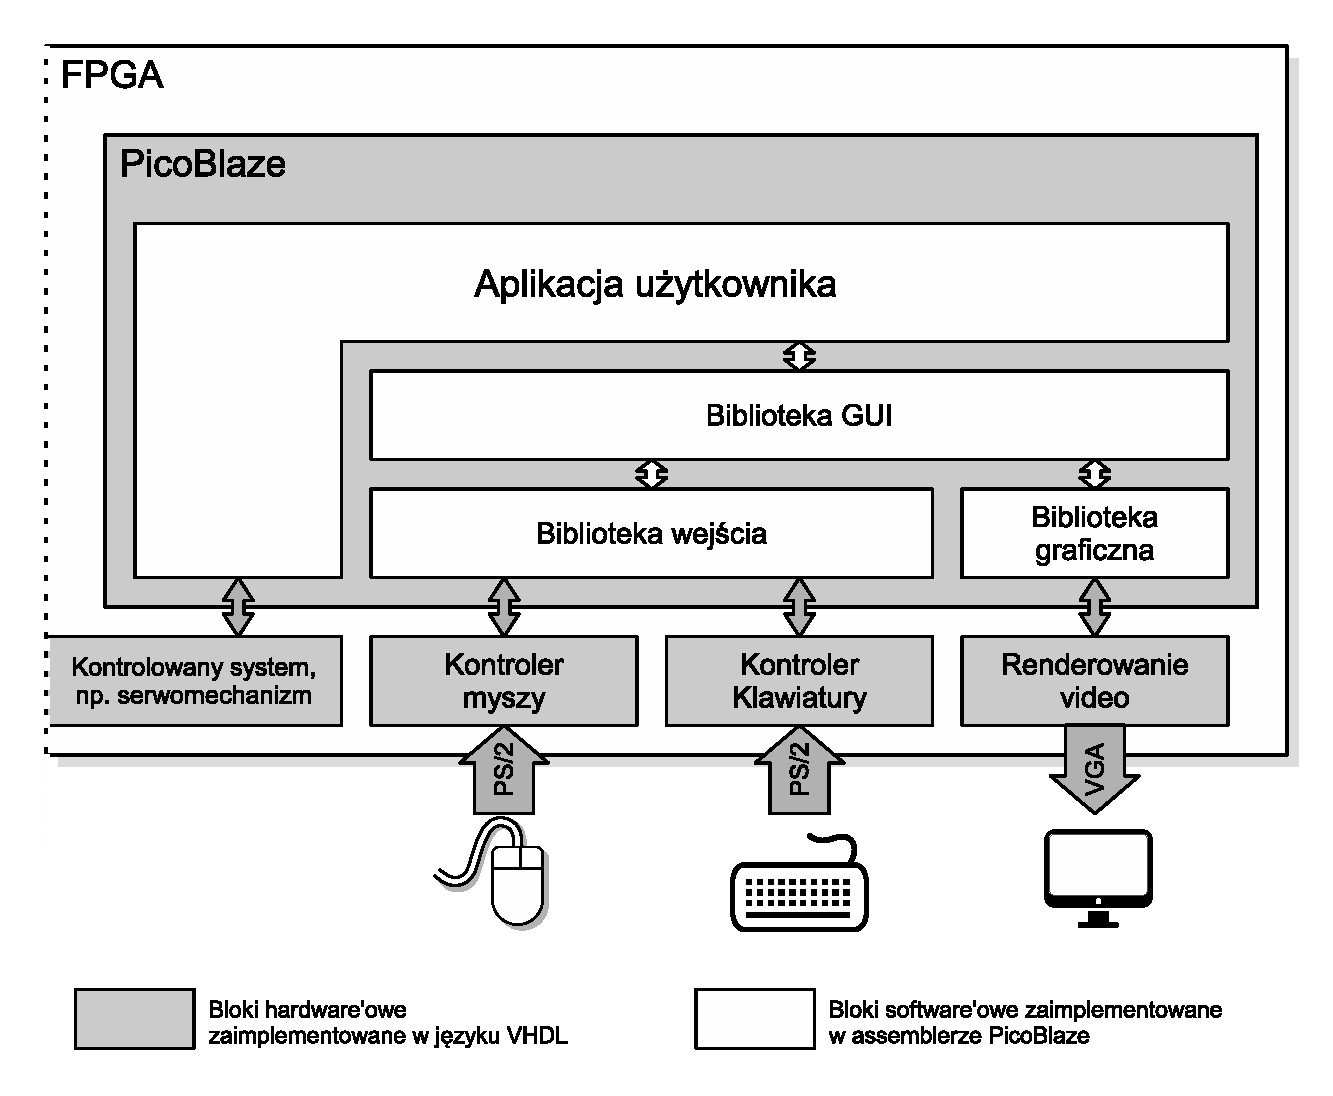
\includegraphics[width=16cm]{obrazki/struktura.eps}
	\caption{Struktura systemu wykonanego w tej pracy}
	\label{struktura}
\end{figure}

Rysunek \ref{struktura} przedstawia poszczególne części pracy oraz relacje między nimi. Można rozróżnić dwa podstawowe typy elementów:
\begin{itemize}
\item Elementy pracy napisane w języku Verilog, które mają swoją reprezentację w~układzie reprogramowalnym. Są to moduły wejścia-wyjścia stojące między procesorem a urządzeniami peryferyjnymi.
\item Elementy pracy napisane w assemblerze, które są uruchamiane na procesorze PicoBlaze. Są to biblioteki, które kontrolują urządzenia wejścia-wyjścia i~udostępniają programiście prosty sposób obsługi graficznego interfejsu użytkownika.
\end{itemize}

Każde z urządzeń zewnętrznych, które może zostać podpięte do systemu, posiada moduł do jego obsługi zaimplementowany w układzie FPGA. Moduł ten udostępnia porty wejścia-wyjścia dla procesora PicoBlaze. Przy pomocy tych portów biblioteki niskiego poziomu komunikują się z urządzeniami i udostępniają interfejs dla biblioteki wyższego poziomu -- biblioteki GUI. Biblioteka ta udostępnia programiście interfejs, który pozwala na obsługę elementów graficznych na ekranie. Aplikacja użytkownika wykonuje specyficzne dla niej zadania (np. sterowanie serwomechanizmem) i dodatkowo wykorzystuje bibliotekę GUI w celu komunikacji z operatorem.

